\chapter{Etapas del proyecto: división en sprints y seguimiento de los mismos}\label{chapter:sprints}
\addcontentsline{toc}{chapter}{Etapas del proyecto: división en sprints}

El proyecto se ha dividido en diez sprints de dos semanas cada uno. Además, durante el transcurso de cada sprint se ha realizado un seguimiento del trabajo realizado en el mismo, aportando \emph{burndown charts} de cada uno de ellos.

Un \emph{burdown chart} es una gráfica en la que se muestra el progreso de un proyecto durante cierto periodo de tiempo preestablecido (un sprint, una release o el proyecto completo, por ejemplo). Para la construcción de los mismos se requieren los siguientes elementos:
\begin{itemize}
\item El periodo de \emph{tiempo a analizar}, que se corresponderá con el eje X de la gráfica. El inicio del periodo temporal vendrá representado por $x = 0$ mientras que el final del periodo temporal será representado por $x = t$ donde $t$ es la duración del periodo. Si observamos el burndown chart global del proyecto (Figura global), estos dos valores se corresponderán, respectivamente, con las fechas de inicio y finalización del mismo.
\item La cantidad de trabajo a realizar, que se corresponderá con el eje Y de la gráfica y representa el trabajo planificado que se deberá realizar en el periodo de tiempo a analizar. Cuando se realiza la estimación de las tareas, independientemente de la unidad de estimación empleada, se obtiene una cantidad de trabajo a realizar (en horas, por ejemplo). Así pues, la cantidad de trabajo restante irá decreciendo conforme el tiempo vaya avanzando.
\item Una referencia ideal, que será la línea diagonal trazada desde la esquina superior izquierda hasta la esquina inferior derecha de la gráfica. Se trata de una representación de la relación ideal entra la disminución de la cantidad de trabajo y el tiempo dedicado durante el transcurso de la fase correspondiente. Esto es, cuanto más se aproxime la línea real a la ideal se estará trabajando de mejor manera en relación a la consecución de los objetivos marcados.
\end{itemize}

Adicionalmente, si se poseen conocimientos y experiencia trabajando con herramientas ágiles, se puede obtener información útil sobre el seguimiento del proyecto con el fin de impulsar buenas prácticas e impulsar el desarrollo del mismo.

\section{Análisis de cada sprint}

\begin{figure}[H]
\centering
\subfloat[Burndown chart del sprint 1 (periodo del al ).]{\label{fig:sprint1}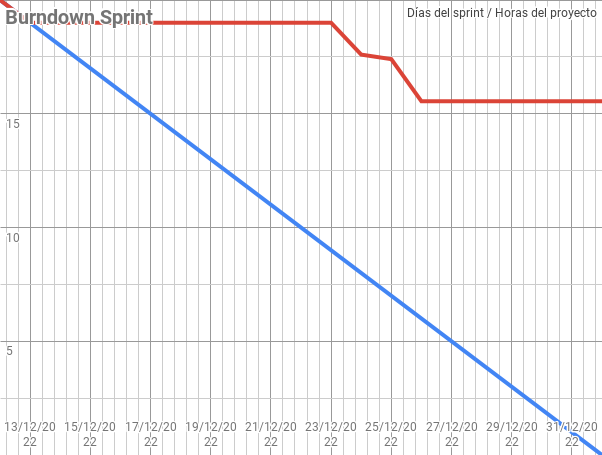
\includegraphics[width=0.46\textwidth]{sprints/Burndown Sprint 1.png}}\qquad
\subfloat[Burndown chart del sprint 2 (periodo del al ).]{\label{fig:sprint2}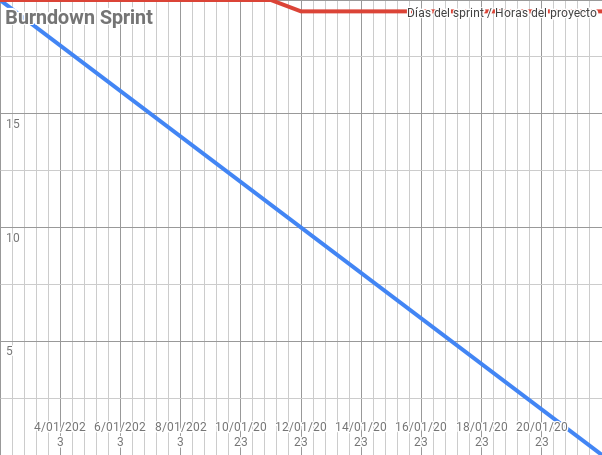
\includegraphics[width=0.46\textwidth]{sprints/Burndown Sprint 2.png}}\qquad
\subfloat[Burndown chart del sprint 3 (periodo del al ).]{\label{fig:sprint3}
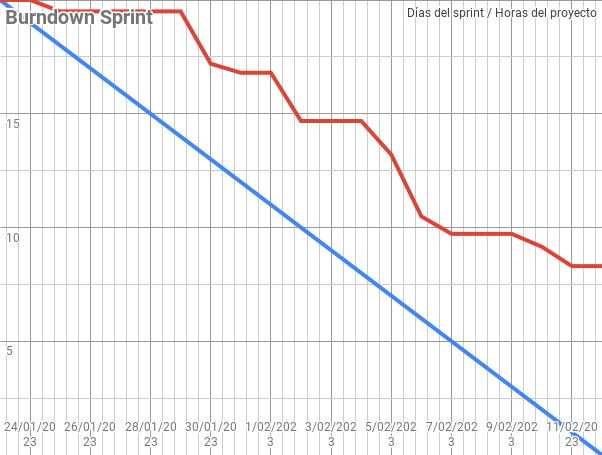
\includegraphics[width=0.46\textwidth]{sprints/Burndown Sprint 3.png}}\qquad
\subfloat[Burndown chart del sprint 4 (periodo del al ).]{\label{fig:sprint4}
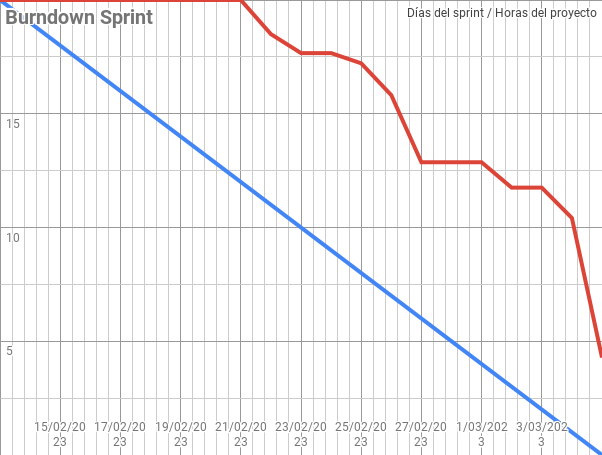
\includegraphics[width=0.46\textwidth]{sprints/Burndown Sprint 4.png}}\qquad
\subfloat[Burndown chart del sprint 5 (periodo del al ).]{\label{fig:sprint5}
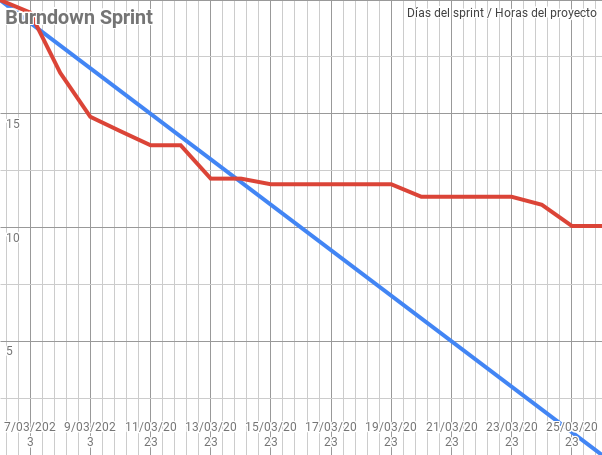
\includegraphics[width=0.46\textwidth]{sprints/Burndown Sprint 5.png}}\qquad
\subfloat[Burndown chart del sprint 6 (periodo del al ).]{\label{fig:sprint6}
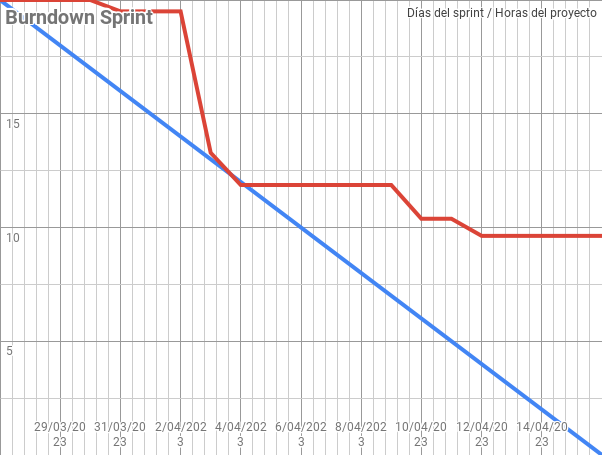
\includegraphics[width=0.46\textwidth]{sprints/Burndown Sprint 6.png}}
\caption{Burdown charts de los seis primeros sprints del proyecto.}
\label{fig:sprints1-6}
\end{figure}

\subsection{Sprint 1 (Figura \ref{fig:sprint1})}

Este primer sprint representa una situación anómala que no se debería dar. La explicación es sencilla: las líneas rojas horizontales representan periodos de tiempo en los cuales no se ha estado trabajando en el proyecto. No obstante, esto es correcto puesto que aunque se definieron unos objetivos al principio, todavía no tenía claro el procedimiento a seguir para la consecución de los mismos. Aunque podría haberse omitido este periodo de seguimiento, se ha decidio incluirlo como muestra de una tendencia no deseable en relación al desarrollo de un proyecto.

\subsection{Sprint 2 (Figura \ref{fig:sprint2})}

En este segundo sprint tampoco se ha alcanzado 
\subsection{Sprint 3 (Figura \ref{fig:sprint3})}
\subsection{Sprint 4 (Figura \ref{fig:sprint4})}
\subsection{Sprint 5 (Figura \ref{fig:sprint5})}
\subsection{Sprint 6 (Figura \ref{fig:sprint6})}
\subsection{Sprint 7}
\subsection{Sprint 8}
\subsection{Sprint 9}
\subsection{Sprint 10}

\section{Análisis global del proyecto}